\chapter{Charge électrique}

\section{Propriétés de la charge électrique}

\marginnote{
  Tremblay \S 1.1 à 1.6

  Lafrance \S 1.1 et 1.2
}

\minisec{Objectif}

\begin{enumerate}
  \item L'étudiant saura qu'il existe deux types de charges électriques et
    comprendra quelles expériences permettent de le démontrer.
  \item L'étudiant connaîtra le principes de conservation de la charge et saura
    l'appliquer pour résoudre des problèmes simples.
  \item L'étudiant connaîtra le principe de quantification de la charge et
    pourra l'appliquer pour résoudre des problèmes simples.
  \item L'étudiant comprendra la polarisation induite dans les isolants.
\end{enumerate}


\minisec{Matériel}

\begin{enumerate}
  \item Tige de plastique
  \item Tige de verre
  \item Tige métallique
  \item Laine
  \item Fourrure
\end{enumerate}


\marginnote{10 minutes}
\minisec{Démonstration de l'existence de deux types de charges}

\begin{enumerate}
  \item Si on approche les deux tiges de plastique, rien ne se produit.
  \item Si on frotte les deux tiges de plastique avec de la laine, elles se
    repoussent. Comme les deux tiges ont subi le même traitement, elles ont la
    même \textbf{charge}. Donc, \textbf{les charges identiques se repoussent}.
  \item On répète avec les tiges de verre qu'on frotte avec la fourrure.
  \item On frotte une tige de plastique et une tige de verre, elles s'attirent.
    Il semble donc que la charge de la tige de verre soit différente de celle
    de plastique et que \textbf{les charges opposées s'attirent}.
  \item Si on approche la laine qui a chargé le plastique de la tige de verre,
    elles se repoussent. Par conséquent la tige de plastique a transféré ses
    charges à la laine qui acquiert donc une charge identique à celle de la
    tige de verre.
  \item Si on approche un objet métallique non chargé de la tige de plastique
    chargée, on constate une attraction. Le métal se charge par
    \textbf{induction} et l'extrémité proche de la tige de plastique acquiert
    une charge opposée à celle du plastique.
\end{enumerate}


\minisec{Propriétés de la charge électrique}
\marginnote{5 minutes}
\vspace{2mm}

\begin{fondamentalbox}
  Il existe deux types de charges électriques
  \begin{itemize}
    \item la charge \textbf{positive} (celle du verre);
    \item la charge \textbf{négative} (celle du plastique).
  \end{itemize}

  Les objets possédant une charge électrique exercent une force les uns sur les
  autres:
  \begin{itemize}
    \item deux objets avec le même type de charge se repoussent;
    \item deux objets avec des charges opposées s'attirent.
  \end{itemize}
\end{fondamentalbox}

On notera souvent les charges électriques par des $q$ : $q$, $Q$, $q_1$, $q_2$,
\ldots.

L'unité SI pour la charge est le \textbf{coulomb} (C). La \textbf{charge
élémentaire} est la charge du proton et vaut
$$e = \SI{1.602 176 634e-19}{\coulomb}.$$
\marginnote{
  Valeur exacte décidée le 16 novembre 2018, en application à partir du 20 mai
  2019
}
L'électron a une charge de $-e$.

\begin{fondamentalbox}
  Au centre d'un atome se trouve un noyau dense contenant des protons chargés
  positivement et des neutrons sans charge électrique. Un nuage d'électrons
  chargés négativement entoure le noyau.
\end{fondamentalbox}

Lorsqu'on charge par frottement, ce sont les électrons qui sont arrachés d'un
matériau et transféré à l'autre. Les protons sont \og cachés \fg\ au centre des
atomes.

Un objet \textbf{neutre} a autant de protons que d'électrons. La plupart des
objets dans l'univers sont neutres.


\begin{diapobox}
  \minisec{Question}
  \marginnote{5 minutes}

  Un téléphone d'une marque connue a une batterie d'une capacité de
  \SI{6556}{C}.  Combien d'électrons peuvent être déplacés par cette batterie?

\end{diapobox}

\begin{reponsebox}
  Il suffit de diviser la charge totale que peut déplacer la batterie par la
  charge d'un seul électron
  \[
    \frac{\SI{6556}{C}}{\SI{1.602e-19}{C}} = \num{4.092e22} =
      \SI{67.95}{\milli\mole}
  \]
\end{reponsebox}


\begin{fondamentalbox}
  \minisec{Principe de conservation de la charge}
  \marginnote{10 minutes}
  La charge électrique totale dans un système fermé est toujours la même.
\end{fondamentalbox}

Par exemple, la charge est conservée lors de la désintégration d'un neutron
libre (temps de demi-vie d'environ \SI{10.3}{minutes}):
\[ n \rightarrow p^+ + e^- + \bar{\nu}_e. \]


\marginnote{
  5 minutes

  \includegraphics[width=3cm]{01-force-electrique/figures/fission.png}
}
\begin{diapobox}
  \minisec{Question}

  Dans un réacteur nucléaire typique, un neutron lent entre en collision avec
  un noyau d'uranium ce qui provoque la fission du noyau en deux noyaux plus
  petits:
  \[
    \ce{n + ^235U -> 3n + ^141Ba + ^AX}
  \]
  Quel est le noyau X?
\end{diapobox}

\begin{reponsebox}
  On détermine la charge au départ: le neutron a une charge nulle, l'uranium a
  92 protons. La charge initiale est donc $92e$. Après la fission, on a trois
  neutrons qui ne contribuent pas à la charge, un noyau de barium qui a 56
  protons et un noyaux mystère avec $Z$ protons. La charge finale est donc $(Z
  + 56)e$. Par le principe de conservation de la charge, la charge initiale et
  la charge finale doivent être égales d'où
  \begin{align*}
    92e &= (Z + 56)e  \\
      Z &= 36
  \end{align*}
  Le noyau $X$ est donc du krypton, Kr. Si on ajoute le principe de
  conservation du nombre de masse, on peut aussi déduire que la masse du
  krypton doit être de 92: \ce{^AX = ^92Kr}.
  \vspace{-1mm}
\end{reponsebox}


\begin{diapobox}
  \minisec{Question}
  \marginnote{10 minutes}

  Indiquez si chacune des réactions suivantes est possible.
  \begin{enumerate}
    \item \ce{H^+ + OH^- -> H_2O}
    \item $\pi^+ + p^+ \longrightarrow \Sigma^0 + K^+$
    \item \ce{^4_2He^{2+} + ^14_7N -> ^17_8O + p^+}
  \end{enumerate}
\end{diapobox}


\begin{fondamentalbox}
  \minisec{Quantification de la charge}
  \marginnote{5 minutes}

  La charge électrique ne peut prendre que des valeurs qui correspondent à des
  multiples entier de la charge élémentaire.
\end{fondamentalbox}

Par exemple, on peut avoir des charges de $e$, $10^{8}e$, $-45e$, etc. On ne
peut pas avoir une charge de $0.1e$, $-\frac{1}{2}e$ ou $\num{3.51e-4}e$.


\begin{diapobox}
  \minisec{Question}
  \marginnote{10 minutes}
  Est-ce qu'un objet peut avoir les charges suivantes?

  \begin{enumerate}
    \item $q_0 = \SI{0.452e-19}{C}$
    \item $q_1 = \SI{-2.05056e-17}{C}$
    \item $q_2 = \SI{3.74868e-18}{C}$
    \item $q_3 = \SI{4.00}{C}$
  \end{enumerate}
\end{diapobox}

\begin{reponsebox}
  La charge $q_0$ est inférieure à la charge élémentaire, donc impossible. La
  charge $q_1$ est 128 fois la charge d'un électron, donc c'est possible. $q_2$
  est $23.4e$, donc impossible. Finalement, la charge $q_3$ est tellement
  grande, qu'à moins qu'on puisse faire une mesure précise jusqu'à la 19e
  décimale, on peut, à toute fin pratique, considérer que cette charge est
  possible.
\end{reponsebox}


\sectionline

\clearpage


\section{Isolants et conducteurs}
\marginnote{
  10 minutes

  Tremblay \S 1.7 et 1.8

  Lafrance \S 1.3
}
Lorsqu'on frotte une tige de verre ou de plastique, des électrons sont arrachés
à un des matériaux et transférés sur l'autre. L'énergie pour arracher les
électrons est fournies par la personne qui frotte. Nous avons vu qu'un objet
métallique est attiré par une tige de plastique chargée. Dans un métal, des
électrons sont libres de se déplacer (environ un électron par atome) ce qui
leur permet de se réorganiser dans le matériau lorsqu'ils ressentent une force
électrique externe.  La tige métallique n'a pas été frottée mais elle attire
néanmoins la tige de plastique chargée.

On dit qu'on a \textbf{induit} une redistribution de la charge dans un métal
en approchant un objet chargé. Aucune charge n'est transférée entre les deux
objets.


\begin{diapobox}
  \minisec{Question}
  \marginnote{5 minutes}

  On induit une séparation de charge dans une tige métallique en approchant une
  tige de plastique chargée. Comment sont disposées les charges dans la tige
  métallique?
  \begin{center}
    \includegraphics[scale=0.5]{01-force-electrique/figures/tige-chargee.pdf}
  \end{center}
  \begin{enumerate}
    \item \includegraphics[scale=0.5]{01-force-electrique/figures/tige.pdf}
      \hspace{-1.3cm}\tikz \node at (-10, 0) {$---$};
    \item \includegraphics[scale=0.5]{01-force-electrique/figures/tige.pdf}
      \hspace{-1.3cm}\tikz \node at (-10, 0) {$+++$};
      \hspace{-2.8cm}\tikz \node at (-10, 0) {$+++$};
    \item \includegraphics[scale=0.5]{01-force-electrique/figures/tige.pdf}
      \hspace{-1.3cm}\tikz \node at (-10, 0) {$---$};
      \hspace{-2.8cm}\tikz \node at (-10, 0) {$+++$};
    \item \includegraphics[scale=0.5]{01-force-electrique/figures/tige.pdf}
      \hspace{-1.3cm}\tikz \node at (-10, 0) {$+++$};
    \item \includegraphics[scale=0.5]{01-force-electrique/figures/tige.pdf}
      \hspace{-1.3cm}\tikz \node at (-10, 0) {$+++$};
      \hspace{-2.8cm}\tikz \node at (-10, 0) {$---$};
  \end{enumerate}
\end{diapobox}


Un \textbf{conducteur} est un matériau dans lequel les charges peuvent se
déplacer rapidement. Un \textbf{isolant} est un matériau dans lequel les
charges ont beaucoup de difficulté à se déplacer.

La différence entre les deux types est le \textbf{temps de relaxation},
c'est-à-dire le temps que des charges mettent à se déplacer jusqu'à leur
position d'équilibre.

Exemple: cuivre \SI{1e-12}{\second}, verre \SI{2}{\second}, polystyrène
\SI{1e10}{\second}.


\begin{diapobox}
  \minisec{Question}
  \marginnote{
    5 minutes

    Électroscope
  }
  Que se passe-t-il si on touche la partie du haut avec une tige chargée
  négativement puis qu'on la retire?
  \begin{center}
    \includegraphics[scale=0.3]{01-force-electrique/figures/electroscope.png}
  \end{center}
\end{diapobox}
\begin{reponsebox}
  Une partie des électrons excédentaires sur la tige seront transférés à
  l'électroscope lors du contact. Par conséquent, l'électroscope aura une
  charge nette négative. Les deux feuillets de l'électroscope, avec des charges
  de même signe, se repousseront. Puisque les électrons n'ont nulle part où
  aller, ils demeureront sur l'électroscope et les feuillets demeureront
  écartés.
\end{reponsebox}


\minisec{Objets conducteurs identiques en contact}
\marginnote{3 minutes}
Si deux objets conducteurs identiques sont mis en contact, les charges qu'ils
portaient seront très rapidement réparties également entre les deux objets.

\begin{diapobox}
  \minisec{Question}
  \marginnote{10 minutes}
  Deux fourchettes métalliques identiques ont des charges $Q$ et $-6Q$,
  respectivement. Les deux fourchettes sont mises en contact puis sont
  séparées.  Quelles sont les charges sur chacune des fourchettes?
\end{diapobox}

\begin{reponsebox}
  La charge totale dans le système avant le contact est $Q + -6Q = -5Q$.

  Par le principe de conservation de la charge, la charge totale après le
  contact sera aussi de $-5Q$.

  Puisque les deux fourchettes sont des conducteurs, les charges (électrons)
  pourront se déplacer d'une à l'autre.

  Puisque les fourchettes sont identiques la charge sur chacune d'elle après le
  contact doit être la même.

  Par conséquent, elles ont chacun la moitié de la charge totale, soit
  $-\num{2.5}Q$.
\end{reponsebox}


\minisec{Polarisation dans les isolants}
\marginnote{
  10 minutes

  Ballon
}

Comment un ballon qu'on frotte sur ses cheveux peut-il tenir au mur si le
ballon et le mur sont des isolants?

Le ballons est chargé par frottement et acquiert une charge négative. Le mur
est neutre et isolant, donc les électrons ne sont pas libres de se déplacer.
Par contre, les atomes à proximité du ballon vont se réorganiser très
légèrement : le nuage d'électron s'éloignera du ballon alors que le noyau
s'en rapprochera. Les atomes seront \textbf{polarisés}. Puisque le ballon est
plus près des charges positives que des charges négatives, il y a une
attraction nette entre le ballon et le mur.

\begin{diapobox}
  Le coefficient de frottement entre le mur et le ballon est $\num{0.6}$, et la
  masse du ballon est de \SI{2.9}{g}. Quel est le module de la force électrique
  entre le ballon et le mur?
  \begin{center}
  \begin{tikzpicture}
    \draw (3, 1.7) -- (3, -1.9);
    \draw (2.298, -1.928) arc (-40:40:3);
    \draw[
      decorate,
      decoration={
        markings, mark=between positions 0 and 1 step 8mm with {
          \node[circle, negative, minimum size=4mm] (0, 0) {$-$};
        }
      }
    ]
      (1.915, -1.607) arc (-40:40:2.5);
    \foreach \y in {1.7, 0.9, 0.1, -0.7, -1.5} {
      \draw[positive] (3.7, \y) arc (90:270:0.5 and 0.3) -- (3.7, \y);
      \node at (3.5, \y - 0.3) {$+$};
      \draw[negative] (3.71, \y - 0.6) arc (-90:90:0.5 and 0.3) -- (3.71, \y - 0.6);
      \node at (3.9, \y - 0.3) {$-$};
    }
    \coordinate (origin) (0, 0);
    \draw[ultra thick, ->] (origin) -- (-1, 0) node[left] {$\vec{N}$};
    \draw[ultra thick, ->] (origin) -- (1, 0) node[right] {$\vec{F}_e$};
    \draw[ultra thick, ->] (origin) -- (0, 1.4) node[right] {$\vec{f}$};
    \draw[ultra thick, ->] (origin) -- (0, -1.4) node[right] {$\vec{F}_g$};
    \draw[draw=white,fill=white] (-0.02, -0.02) rectangle (0.02, 0.02);
    \node at (-1, 1.7) {Ballon};
    \node at(6, 1.7) {Mur};
  \end{tikzpicture}
  \end{center}
\end{diapobox}

\begin{reponsebox}
  On suppose que le ballon est à l'équilibre, donc $F_e = N$ et $f = F_g$. Par
  conséquent, $f = mg$. Si on suppose que le frottement est le frottement
  statique maximum, autrement dit le ballon est sur le point de tomber, alors
  on a que $f = \mu_s N = \mu_s F_e$. Donc
  \[
    F_e = \frac{mg}{\mu_s} = \SI{47.37}{mN}
  \]
\end{reponsebox}

On peut aussi voir le même phénomène en attirant des morceaux de papier avec un
bout de plastique chargé. Le bout de plastique chargé induit une polarisation
dans le papier et le papier est attiré par le plastique.

\begin{diapobox}
  \minisec{Vidéo}

  Le vidéo \texttt{polarisation-isolant-attraction.mov} montre un morceau de
  \textit{spaghetti} frotté sur des cheveux (donc chargé négativement) qui
  attire des morceaux de pitas secs.
\end{diapobox}

% L'exercice suivant est déplacé dans le TP1.
%\minisec{Exercice}
%\marginnote{5 minutes}
%Le coefficient de frottement entre le mur et le ballon est $0.6$, et la masse
%du ballon est de \SI{2.9}{g}. Quel est
%le module de la force électrique entre le ballon et le mur?

%\minisec{Solution de l'exercice}
%\marginnote{15 minutes}

%$N = F_e$ car composante horizontale de l'accélération est nulle (équilibre).

%$f = \mu_s N = \mu_s F_e$.

%$f = F_g$ car composante verticale de l'accélération est nulle (équilibre).

%$\mu_s F_e = mg$

%$F_e = \frac{mg}{\mu_s} = \SI{0.0474}{N}$


\minisec{Charge par induction}
\marginnote{5 minutes}
Nous avons parlé de charge par frottement. Il est également possible de
charger un conducteur par induction.
\begin{center}
  \includegraphics[height=3cm]{01-force-electrique/figures/charge-induction-3.pdf}
\end{center}
On approche une tige chargée négativement du conducteur, sans lui toucher. La
présence de la tige chargée créera une séparation de charge dans le conducteur
par induction.  On relie le côté du conducteur le plus éloigné de la tige à la
\textit{terre}.  C'est ce qu'on appelle une \textbf{mise à la terre}. Le
surplus d'électrons qui s'étaient déplacés de ce côté parce qu'ils étaient
repoussés par les électrons de la tige pourront aller à la terre. On déconnecte
ensuite la mise à la terre, puis, on éloigne la tige chargée. Il reste une
charge nette positive sur le conducteur.


\sectionline
\newpage

\section{Loi de Coulomb}

%\minisec{Matériel}

%\begin{enumerate}
  %\item Balance à torsion pour loi de Coulomb
%\end{enumerate}


%\subsection*{Démonstration de la loi de Coulomb}
%\marginpar{15 minutes}
%\marginpar{Montage installé au labo}

  %Une boule métallique installée sur une balance à torsion.

  %Faire les manips suivantes dans l'ordre.

  %\begin{itemize}
    %\item Boules non chargées, mesurer position du laser et distance entre les
      %boules
    %\item Une boule chargée, mêmes mesures. La boule suspendue devrait se
      %rapprocher de la boule fixe puisqu'elle se polarise par induction.
    %\item Deux boules chargées. La boule suspendue devrait s'éloigner de la
      %boule fixe car des charges de même signe se repoussent. Disons que la
      %distance entre les boules est $r$ et la position du laser s'est déplacée
      %de $d$.
    %\item Si on déplace la boule fixe à $2r$, la force de répulsion entre les
      %deux boules diminue d'un facteur $4$ et le laser devrait être à une
      %distance $d/4$ de sa position d'équilibre.
    %\item On remet la boule fixe à sa position initiale,$r$. On touche la boule
      %fixe avec une troisième boule identique qu'on retire. La charge de la boule fixe passe
      %donc de $Q$ à $Q/2$. La force entre les deux boules diminue donc de
      %moitié et on devrait voir le pointeur laser se déplacer à $d/2$.
  %\end{itemize}

\marginnote{
  Tremblay \S 1.9

  Lafrance \S 1.4
}

\minisec{Objectif}

\begin{enumerate}
  \item L'étudiant comprendra la loi de Coulomb et comment cette loi capture
    toutes les observations faites précédemment au sujet des charges.
  \item L'étudiant pourra faire des calculs de forces électrostatiques.
  \item L'étudiant comprendra le principe de superposition.
\end{enumerate}


\minisec{Observations clés}
\marginnote{10 minutes}
\begin{itemize}
  \item charges opposées s'attirent
  \item charges de même signe se repoussent
  \item plus la charge est grande, plus la force est grande
  \item plus les charges sont éloignées, plus la force est petite
\end{itemize}

La loi de Coulomb capture tous ces éléments.

Considérons deux charges $q_1$ et $q_2$ séparées d'une distance $r$.
\begin{center}
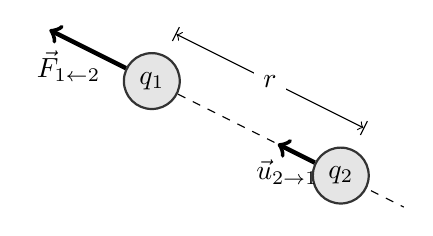
\begin{tikzpicture}[
  charge/.style={circle, draw=black!80, fill=black!10, thick}]
  \draw[dashed] (0, 2) -- (4, 0);
  \node[charge] (q1) at (0.8, 1.6) {$q_1$};
  \node[charge] (q2) at (3.2, 0.4) {$q_2$};
  \draw[|<->|] (1.1, 2.2) -- node[fill=white] {$r$} (3.5, 1);
  \draw[ultra thick, ->] (q1) --
    node[near end, below] {$\vec{F}_{1 \leftarrow 2}$} (-0.5, 2.25);
  \draw[ultra thick, ->] (q2) -- node[near end, below]
  {$\vec{u}_{2 \rightarrow 1}$} (2.4, 0.8);
\end{tikzpicture}
\end{center}
On doit avoir
\begin{eqnarray*}
  F_{1 \leftarrow 2} & \propto & \abs{q_1}, \\
  F_{1 \leftarrow 2} & \propto & \abs{q_2}, \\
  F_{1 \leftarrow 2} & \propto & \frac{1}{r^\gamma}.
\end{eqnarray*}
Autrement dit,
$$
  F_{1 \leftarrow 2} = \frac{k\abs{q_1 q_2}}{r^\gamma}.
$$
où $k$ est une constante de proportionnalité. L'exposant peut être trouvé
expérimentalement. C'est ce qu'à fait Charles Augustin de Coulomb. L'exposant
est $2$, soit le même que celui qui apparaît dans la loi de la gravitation
newtonienne.

Pour spécifier l'orientation, nous utilisons un vecteur unitaire $\vec{u}_{2
\rightarrow 1}$ qui pointe de la charge $q_2$ vers la charge $q_1$. Si les
deux charges sont de même signe, la force est répulsive et la force sur $q_1$
est dans la même direction que $\vec{u}_{2 \rightarrow 1}$. On note que
$q_1q_2$ est positif. Donc
\begin{fondamentalbox}
  \textbf{Loi de Coulomb}

  \[
    \vF_{1 \leftarrow 2} = \frac{kq_1q_2}{r^2}\vec{u}_{2 \rightarrow 1}
  \]
\end{fondamentalbox}

On peut facilement trouver les unités de $k$ par analyse dimensionnelle. La
valeur est déterminée expérimentalement:
$$k = \frac{1}{4\pi\epsilon_0} = \SI{8.99e9}{N m^2 / C^2}$$
La constante de proportionalité $k$ est reliée à une constante fondamentale de
l'Univers qu'on appelle la \textbf{constante électrique} ou la
\textbf{permittivité du vide} $\epsilon_0$.
$$\epsilon_0 = \SI{8.854e-12}{C^2 / N m^2}$$


\begin{fondamentalbox}
  \minisec{Principe de superposition}
  Si plusieurs charges $q_1, q_2, \ldots, q_N$ et agissent sur une charge $Q$,
  alors la force nette sur $Q$ est la somme des forces exercées par chacune des
  charges
  \[
    \vF = \vF_1 + \vF_2 + \ldots + \vF_N
  \]
\end{fondamentalbox}


\begin{diapobox}
  Vous vous tenez à \SI{2}{m} de votre ami. Combien d'électrons devez vous lui
  transférer pour que la force électrique entre vous deux ait la même grandeur
  que votre poids?
\end{diapobox}

\begin{reponsebox}
  Votre poids a une grandeur $mg$. Si vous transférez $n$ électrons à votre
  ami, votre charge devient $ne$ et la charge de votre ami devient $-ne$. Par
  conséquent la grandeur de la force électrique est
  \begin{align*}
    F_e = \frac{kn^2e^2}{r^2}
  \end{align*}
  On veut
  \begin{align*}
    \frac{k n^2 e^2}{r^2} &= mg  \\
    n &= \sqrt{\frac{mgr^2}{k e^2}}  \\
      &= \sqrt{\frac{mg}{k}} \frac{r}{e}  \\
  \end{align*}
  Supposons que votre masse est $m = \SI{60}{\kilo\gram}$. Alors
  \begin{align*}
    n &= \sqrt{\frac{\SI{60}{kg} \cdot \SI{9.8}{m\per s^2}}{\kval}}
         \frac{\SI{2}{m}}{\eval}  \\
      &= \num{3.193e15}
  \end{align*}
  C'est l'équivalent d'une charge de \SI{0.5115}{mC}.
\end{reponsebox}


\begin{diapobox}
  \minisec{Question}
  On considère une charge négative $q_1$ et une charge positive $q_2$.
  \marginnote{
    \includegraphics[scale=0.4]{01-force-electrique/figures/coulomb-direction.png}
  }

  Dans quelle direction est la force de $q_1$ sur $q_2$, $\vF_{2 \leftarrow 1}$?

  Dans quelle direction est la force de $q_2$ sur $q_1$, $\vF_{1 \leftarrow 2}$?
  
  Dans quelle direction est le vecteur $\vu_{1 \rightarrow 2}$?

  Dans quelle direction est le vecteur $\vu_{2 \rightarrow 1}$?
\end{diapobox}


\begin{diapobox}
  \minisec{Exemple}
  \marginnote{
    \includegraphics[scale=0.5]{01-force-electrique/figures/exercice-membrane.png}
  }
  Un ion \ce{Na+} et un ion \ce{PO4^3-} se trouvent de part et d'autre
  d'une membrane cellulaire. L'épaisseur de la membrane est de \SI{5}{nm} et
  les deux ions sont décalés de \SI{10}{nm} l'un par rapport à l'autre le long
  de la membrane. Quelle est la force exercée par le sodium sur le phosphate?
\end{diapobox}

\begin{reponsebox}
  On peut placer l'origine du système de coordonnées de telle sorte que la
  position du sodium soit $\vr_\mathrm{Na} = 0\xhat + 2d\yhat$ et la position du
  phosphate soit $\vr_\mathrm{PO} = d\xhat + 0\yhat$. Par la loi de Coulomb
  \[
    \vF_\mathrm{PO} =
      \frac{kq_\mathrm{Na}q_\mathrm{PO}}{r^2}
      \vu_{\mathrm{Na}\rightarrow \mathrm{PO}}
  \]
  On sait que $q_\mathrm{Na} = e$ et $q_\mathrm{PO} = -3e$, donc
  \[
    \vF_\mathrm{PO} = \frac{-3ke^2}{r^2}
      \vu_{\mathrm{Na}\rightarrow \mathrm{PO}}
  \]
  Le vecteur unitaire est
  \begin{align*}
    \vu_{\mathrm{Na}\rightarrow \mathrm{PO}} &=
      \frac{\vr_\mathrm{PO} - \vr_\mathrm{Na}}
           {\abs{\vr_\mathrm{PO} - \vr_\mathrm{Na}}}  \\
    &= \frac{d\xhat - 2d\yhat}{r}
  \end{align*}
  Donc
  \begin{align*}
    \vF_\mathrm{PO} = \frac{-3kde^2}{r^3}\left(\xhat - 2\yhat\right)
  \end{align*}
  On peut trouver $r$ simplement à l'aide du théorème de Pythagore
  \[
    r = \sqrt{(2d)^2 + d^2} = \sqrt{5}d
  \]
  Donc
  \begin{align*}
    \vF_\mathrm{PO} = \frac{-3ke^2}{5^{3/2} d^2}\left(\xhat - 2\yhat\right)
  \end{align*}
  Il ne reste qu'à calculer la valeur numérique
  \begin{align*}
    \vF_\mathrm{PO} &= \frac{-3 \cdot \SI{8.99e9}{Nm^2\per C^2}
                            \left(\SI{1.602e-19}{C}\right)^2}
                           {5^{3/2} (\SI{5e-9}{m})^2}
                      \left(\xhat - 2\yhat\right)  \\
                    &= \SI{-2.476e-12}{N}
                      \left(\xhat - 2\yhat\right)
  \end{align*}
  C'est une force toute petite, mais on parle de l'interaction entre deux
  atomes, donc on ne s'attend à rien d'énorme. De plus, puisque les deux ions
  ont des charges opposées, on s'attend à ce que la force soit attractive et
  c'est bien ce que le calcul donne.
\end{reponsebox}

\begin{diapobox}
  \minisec{Exercice}
  \marginnote{20 minutes}
  Deux charges immobiles $q = \SI{4.00}{nC}$ et $Q = \SI{-6.00}{nC}$ sont
  situées à \SI{5}{cm} l'une de l'autre.  Où doit-on positionner une troisième
  charge de telle sorte qu'elle soit à l'équilibre?
\end{diapobox}

\begin{reponsebox}
D'abord, on fait un schéma de la situation. Imaginons que la charge qu'on
ajoute est positive. La direction de la force exercée par $q_1$ et $q_2$ dans
différentes régions est indiquée sur la figure.

\begin{center}
\begin{tikzpicture}[
      charge/.style={circle, draw=black!80, fill=black!10, thick}]
  \draw[->] (-2, 0) -- (4, 0) node[below] {$x$};
  \node[circle, positive] (q1) at (0, 0.5) {$q_1$};
  \node[circle, negative] (q2) at (3, 0.5) {$q_2$};
  \node[charge] (q) at (-1.5, 0.5) {$q$};
  \draw (q1|-0,0) -- ++(0, -0.2) node[below] {$0$};
  \draw (q2|-0,0) -- ++(0, -0.2) node[below] {$d$};
  \draw (q|-0,0) -- ++(0, -0.2) node[below] {$x$};
  % Forces by q1
  \draw[ultra thick, ->, positive] (-0.3, 1.2) -- ++(-1, 0);
  \draw[ultra thick, ->, positive] (1, 1.2) -- ++(1, 0);
  \draw[ultra thick, ->, positive] (3.3, 1.2) -- ++(1, 0);
  % Forces by q2
  \draw[ultra thick, ->, negative] (-1.3, 1.5) -- ++(1, 0);
  \draw[ultra thick, ->, negative] (1, 1.5) -- ++(1, 0);
  \draw[ultra thick, ->, negative] (4.3, 1.5) -- ++(-1, 0);
\end{tikzpicture}
\end{center}

À gauche de $q_1$, les deux forces sont opposées et la plus grande charge en
valeur absolue est plus éloignée. Il est possible que les deux forces
s'annulent.

Entre $q_1$ et $q_2$, les deux forces sont dans la même direction : elles ne
peuvent pas s'annuler.

À droite de $q_2$, les deux forces sont opposées et la plus grande charge en
valeur absolue est plus proche. Il est impossible que les deux forces
s'annulent.

On conclut donc que la position recherchée est pour une valeur $x$ négative. La
distance entre la nouvelle charge $q$ et $q_1$ est donc $\abs{x}$ alors que la
distance entre $q$ et $q_2$ est de $d - x$. On peut calculer le module de la
force exercée par $q_1$ et $q_2$ sur $q$ ainsi que les composantes.
\begin{align*}
  F_1 &= \frac{k\abs{q_1q}}{x^2}        &  F_{1x} &= -\frac{kq_1q}{x^2} \\
  F_2 &= \frac{k\abs{q_2q}}{(d - x)^2}  &  F_{2x} &= -\frac{kq_2q}{(d - x)^2}
\end{align*}

La force nette sur $q$ est nulle car on veut que cette particule soit à
l'équilibre.  Par le principe de superposition, la force nette sur $q$ est
\begin{align*}
     F_x &= F_{1x} + F_{2x} \\
         &= 0  \\
  F_{1x} &= -F_{2x} \\
  -\frac{kq_1q}{x^2} &= \frac{kq_2q}{(d - x)^2} \\
  -\frac{q_1}{x^2} &= \frac{q_2}{(d - x)^2} \\
  x^2q_2 + q_1(d - x)^2 &= 0 \\
  x^2q_2 + q_1d^2 - 2q_1dx + q_1x^2 &= 0 \\
  (q_1 + q_2) x^2 - 2 q_1 d x + q_1d^2 &= 0 \\
  x &= \frac{2q_1 d \pm \sqrt{4q_1^2d^2 - 4(q_1 + q_2) q_1 d^2}}{2(q_1 + q_2)}
\end{align*}
Les deux réponses possibles sont $x = \SI{-22.25}{cm}$ et $x = \SI{2.247}{cm}$.
On sait que la particule doit être à gauche de $q_1$, donc la bonne solution
est $x = \SI{-22.25}{cm}$.
\end{reponsebox}


\sectionline


\section{Résumé}

\begin{itemize}
  \item Deux types de charges (positive et négative).
  \item Charges de même signe se repoussent, de signe opposé s'attirent.
  \item Charge est conservée.
  \item Charge est quantifiée.
  \item Dans un conducteur, charges peuvent se déplacer, pas dans un isolant.
  \item Loi de Coulomb.
  \item Principe de superposition des forces.
  \item Trois façons de charger un objet:
    \begin{itemize}
      \item Par frottement (fonctionne bien avec isolants)
      \item Par contact (fonctionne bien avec les conducteurs)
      \item Par induction (fonctionne avec les conducteurs seulement)
    \end{itemize}
\end{itemize}


